\newpage
\section*{Referencias}
\textbf{Básico: }
\begin{itemize}
	\item \textit{Problema 1.} Problema 9 categoría Benjamín, Canguro Matemático (Portugal).
	\item \textit{Problema 2.} Problema 12 Clasificatoria UAN Primer Nivel, 1999.
	\item \textit{Problema 3.} Problema 2 Selectiva UAN Primer Nivel, 1999.
	\item \textit{Problema 4.} Problema 23 Clasificatoria UAN Primer Nivel, 1997.
	\item \textit{Problema 5.} Problema 2 Selectiva UAN Primer Nivel, 1997.
\end{itemize}

\textbf{Avanzado: }
\begin{itemize}
	\item \textit{Problema 1.} Creado
	\item	\textit{Problema 2.} Final UIS nivel avanzado 2020.
	\item	\textit{Problema 3.} Basado en: Canguro Matemático Brasil, problema 11.
	\item	\textit{Problema 4.} \url{https://www.youtube.com/watch?v=a6m_FsyBV9o&ab_channel=AcademiaInternet}
	\item	\textit{Problema 5.} Problema 24 categoría Estudiante, Canguro Matemático (Portugal), 2019.
\end{itemize}

%------------------------------------------------------------------------------------------------------------   
%----------------------------------                        BASICO                       ---------------------------------- 
%------------------------------------------------------------------------------------------------------------ 

\newpage
\section{Nivel Básico}\label{basico:2020_12_septiembre}

\begin{center}
	\fbox{\fbox{\parbox{6in}{\centering
				\textbf{Tiempo mínimo: } 2 horas y 30 minutos.\\
				\textbf{Tiempo máximo: } 3 horas y 30 minutos.\\	
				\textbf{Procedimientos: }Cada problema debe estar resuelto por escrito, en forma detallada, todos los pasos seguidos para su resolución deben estar bien explicados. Se le brindarán unas hojas grapadas, en la \textit{parte de enfrente} de cada hoja debe estar la solución de los problemas, la \textit{parte posterior} no se leerá pero las operaciones y cálculos deben hacerlos allí. \\
				\textbf{Puntaje: }Cada problema vale 50 puntos, son 5, para un total de 250 puntos.
				}}}
\end{center}

\begin{enumerate}
	\item \textbf{(50 puntos)}. En la Figura se muestran 3 cuadrados. Se conocen algunas longitudes como se muestra en la figura. Si el lado del cuadrado más pequeño mide $6cm$ cuánto es el perímetro de toda la figura que forman los tres cuadrados?
	
			\begin{figure}[H]
				\centering
				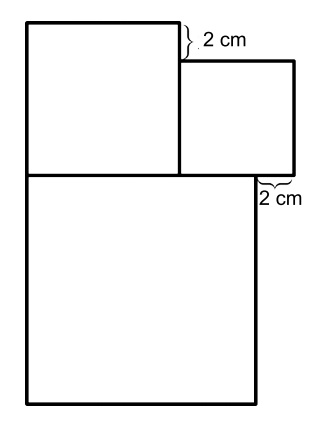
\includegraphics[width=0.4\linewidth]{2020_09_12/imgs/basico_perimetro}
				%\caption{}
				\label{fig:basico_perimetro}
			\end{figure}
			
	\item \textbf{(50 puntos)}. Calcular el resultado de la siguiente suma
	\[
	2\left(1-\frac{1}{2}\right) + 3\left(1-\frac{1}{3}\right) + 4\left(1-\frac{1}{4}\right) + \cdots + 19\left(1-\frac{1}{19}\right) + 20\left(1-\frac{1}{20}\right)
	\]
			
	
	\item \textbf{(50 puntos)}. Oscar escribió en una hoja de papel 5 números enteros positivos y se los mostró a Andrés. Andrés dijo ``La suma de estos 5 números es 23'', y Oscar agregó ``Si! y su producto es 2000. Cuál es el mayor de estos 5 números?''
				

	\item \textbf{(50 puntos)}. Cuántos números de cuatro dígitos mayores que 4000 pueden formarse con los dígitos 2,3,4,5 y 6 si ningún dígito aparece mas de una vez en un número?
			
		
	\item \textbf{(50 puntos)}. Pedro hace la siguiente lista de números
	\[
	1,9,9,7,7,\dots
	\]
	todos los elementos de la lista a partir del quinto elemento son iguales a la cifra de las unidades del producto de los anteriores 4 números de la lista. Por ejemplo el quinto elemento de la lista de Pedro es el 7 porque la cifra de las unidades del producto $1\times 9\times 9\times 7$ es $7$. Pedro continúa así agregando términos a su lista. Cuál es el número que está en la posición $2020$?
\end{enumerate}



%------------------------------------------------------------------------------------------------------------   
%----------------------------------                        AVANZADO                       ---------------------------------- 
%------------------------------------------------------------------------------------------------------------ 

\newpage
\section{Nivel Avanzado}\label{avanzado:2020_12_septiembre}

\begin{center}
	\fbox{\fbox{\parbox{6in}{\centering
				\textbf{Tiempo mínimo: } 2 horas y 30 minutos.\\
				\textbf{Tiempo máximo: } 3 horas y 30 minutos.\\	
				\textbf{Procedimientos: }Cada problema debe estar resuelto por escrito, en forma detallada, todos los pasos seguidos para su resolución deben estar bien explicados. Se le brindarán unas hojas grapadas, en la \textit{parte de enfrente} de cada hoja debe estar la solución de los problemas, la \textit{parte posterior} no se leerá pero las operaciones y cálculos deben hacerlos allí. \\
				\textbf{Puntaje: }Cada problema vale 50 puntos, son 5, para un total de 250 puntos.
	}}}
\end{center}


\begin{enumerate}
	\item \textbf{(50 puntos)}. Hallar todos los valores posibles de $n$ para los cuales se cumple que $n$, $n+2$ y $n+4$ son números primos.
	

	\item \textbf{(50 puntos)}. Considere la función $f(x)$ definida en los enteros positivos. Esta función cumple con la siguiente propiedad:
	\[
	f(xy)=f(x) + f(y)
	\]	
	para cualesquiera enteros positivos $x$ e $y$. Si se sabe que $f(2048)=33$. Calcular el valor de $f(1024)$.
	
	\item \textbf{(50 puntos)}. Cuál es la mayor potencia de $3$ que divide a $25!+26!+27!$?

	\item \textbf{(50 puntos)}. Calcular el área azul en la siguiente figura
	\begin{figure}[H]
		\centering
		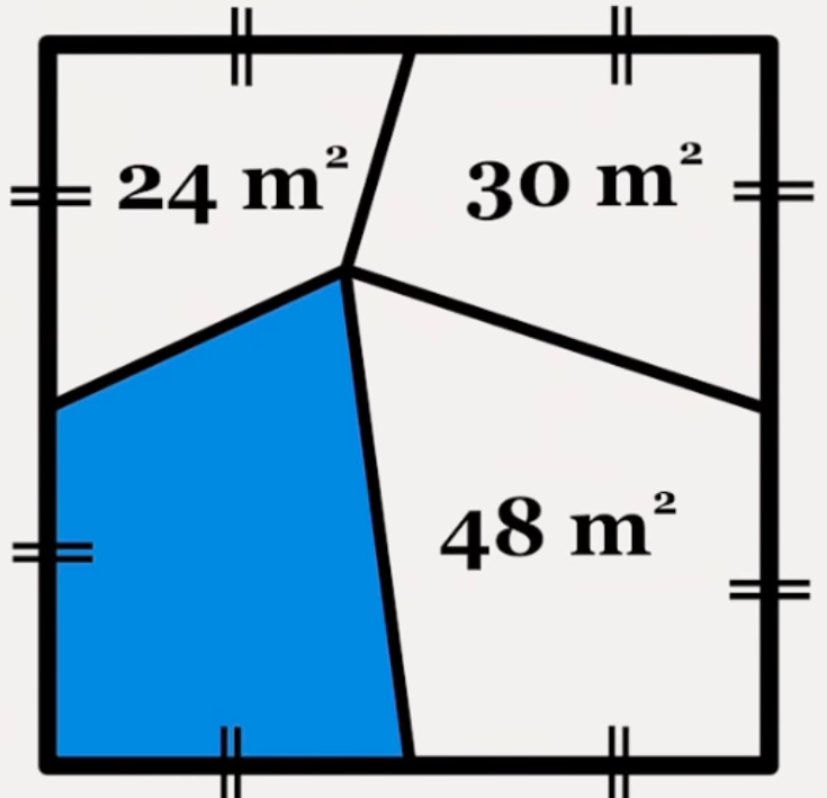
\includegraphics[width=0.4\linewidth]{2020_09_12/imgs/geometria}
		%\caption{}
		\label{fig:geometria}
	\end{figure}


	\item \textbf{(50 puntos)}. Se tiene un cubo. Cuántos planos diferentes existen tales que contengan por lo menos 3 vértices del cubo?

\end{enumerate}